\documentclass[preprint,numbers]{sigplanconf}
% The following \documentclass options may be useful:

% preprint      Remove this option only once the paper is in final form.
% 10pt          To set in 10-point type instead of 9-point.
% 11pt          To set in 11-point type instead of 9-point.
% authoryear    To obtain author/year citation style instead of numeric.
\usepackage[utf8]{inputenc}          % UTF-8 Encoding
\usepackage[british]{babel}          % Use British English language settings
\usepackage{hyperref}                % Interactive PDF
\usepackage{xcolor}                  % Colours
\usepackage[inline]{enumitem}        % Inline enumerations
\usepackage{drawstack}               % Syntactic sugar for tikz for drawing run-time stacks
\usepackage{listings}                % Source code listings

\lstset{
 backgroundcolor=\color{white},   % choose the background color; you must add \usepackage{color} or \usepackage{xcolor}
 basicstyle=\ttfamily\footnotesize,        % the size of the fonts that are used for the code
 keywordstyle=\bfseries,
 commentstyle=\itshape,
 breakatwhitespace=true,         % sets if automatic breaks should only happen at whitespace
 breaklines=true,                 % sets automatic line breaking
 captionpos=b,                    % sets the caption-position to bottom
 escapeinside={\#*}{*\#},          % if you want to add LaTeX within your code
 extendedchars=true,              % lets you use non-ASCII characters; for 8-bits encodings only, does not work with UTF-8
 frame=none,	                   % adds a frame around the code
 keepspaces=true,                 % keeps spaces in text, useful for keeping indentation of code (possibly needs columns=flexible)
 numbers=none,                    % where to put the line-numbers; possible values are (none, left, right)
 rulecolor=\color{black},         % if not set, the frame-color may be changed on line-breaks within not-black text (e.g. comments (green here))
 showspaces=false,                % show spaces everywhere adding particular underscores; it overrides 'showstringspaces'
 showstringspaces=false,          % underline spaces within strings only
 showtabs=false,                  % show tabs within strings adding particular underscores
 tabsize=1,	                   % sets default tabsize to 2 spaces
 title=\lstname,                   % show the filename of files included with \lstinputlisting; also try caption instead of title
 caption={},
 belowcaptionskip=-1\baselineskip,
 xleftmargin=0.1\parindent,
 columns=fullflexible
}

% Define Links as a lst-language
\lstdefinelanguage{Links}{%
  morekeywords={typename, fun, op, var, if, true, false, else, case, switch, handle, handler, shallowhandler, do, sig},%
  sensitive=t, %
  keywordstyle=\color{red},
  emph={Comp,Bool,Int,Char,String,Choose,Return,Toss,Heads,Tails,Nothing,Just,Fail,Zero,Maybe},
  emphstyle={\color{blue}},
  comment=[l]{\#},%
  escapeinside={(*}{*)},%
  morestring=[d]{"}%
}

\newcommand{\textapprox}{{\fontfamily{ptm}\selectfont\texttildelow}}
\newcommand{\wildarrow}{\linksify{\textapprox{}>}}
% Links style
\lstdefinestyle{links}{
  basicstyle=\linespread{1.0}\ttfamily\footnotesize,
  language=Links,
  literate= {~>}{{\wildarrow}}1
}

\lstset{style={links}}

% OCaml style
\lstdefinestyle{ocaml}{
  basicstyle=\linespread{1.0}\ttfamily\footnotesize,
  language=Caml,
  morekeywords={effect}
}

%% TODOs and comments
\newcommand{\msgbox}[2]{{%
  \par\noindent\small\color{red}%
  \framebox{\parbox{\dimexpr\linewidth-2\fboxsep-2\fboxrule}{\textbf{#1:} #2}}%
}}
\newcommand{\todo}[1]{\msgbox{TODO}{#1}}

\newcommand{\sam}[1]{\msgbox{Sam}{#1}}
\newcommand{\dhil}[1]{\msgbox{Daniel}{#1}}
\newcommand{\kc}[1]{\msgbox{KC}{#1}}

\begin{document}
%% Remove SIGPLANCONF copyright space
\makeatletter
\def\@copyrightspace{\relax}
\makeatother

%% Set paper geometry
\special{papersize=8.5in,11in}
\setlength{\pdfpageheight}{\paperheight}
\setlength{\pdfpagewidth}{\paperwidth}

%% Obfuscate e-mail addresses
\newcommand{\camacuk}{@cam.ac.uk}
\newcommand{\edacuk}{@ed.ac.uk}
\newcommand{\contact}[2]{#1@#2}
\newcommand{\reachme}[1]{\hyperlink{mailto:\contact{#1}}{\contact{#1}}}

\titlebanner{DRAFT -- Extended Abstract}    % These are ignored unless
\preprintfooter{} % 'preprint' option specified.

\title{Compiling Effect Handlers}
%\subtitle{-- Extended Abstract --}
\authorinfo{Daniel Hillerström}
           {The University of Edinburgh}
           {~}%{\reachme{daniel.hillerstrom}}

\authorinfo{Sam Lindley}
           {The University of Edinburgh}
           {~}%{\reachme{sam.lindley}}

\authorinfo{KC Sivaramakrishnan}
           {The University of Cambridge}
           {~}

\maketitle

\begin{abstract}
  Algebraic effects and handlers provide a modular abstraction for
  modeling and controlling computational effects. We present a
  compiler for the experimental language Links with effect
  handlers. Our compiler interfaces with the Multicore OCaml backend
  to take advantage of OCaml's implementation of efficient handlers.
\end{abstract}

\section{Motivation}
%\kc{if you find yourself short of space, I'd axe some of this section.}

% \sam{this paragraph needs to be a bit more focused}
% Algebraic effects and effect handlers \cite{Plotkin2013} afford a
% modular and structured interface for programming with delimited
% continuations. In previous work, we extended the functional web
% programming language Links with algebraic effects and handlers
% \cite{Hillerstrom2015,Hillerstrom2016}. Links uses row polymorphism to provide
% extensible effect typing.

Algebraic effects and handlers \cite{Plotkin2013} afford a compelling
and modular alternative to monad transformers for controlling
computational effects. In previous work, we extended the functional
web programming language Links with algebraic effects and handlers
\cite{Hillerstrom2015,Hillerstrom2016}.
% Links uses row polymorphism to provide extensible effect typing.

Links is a single language for multi-tier web-programming
\cite{Cooper2006}. It has three backends:
\begin{enumerate*}[label={\roman*)}]
 \item a JavaScript compiler for the client,
 \item an interpreter for the server,
 \item and an SQL generator for the database.
\end{enumerate*}
Currently effect handlers are only supported on the server; in future
we intend to extend the JavaScript compiler to support them too.

In order to improve performance, and to study efficient compilation of effect
handlers in general, we have implemented a Links compiler that targets the
Multicore OCaml backend \cite{Dolan2015}. By taking advantage of the OCaml
backend we obtain both native code compilation support and the OCaml toolchain
for free.

% \kc{The paper as it stands now does not mention why, but only deals with the
% question of how. We should mention the current Links backends, and say they
% they are only interpreted. The goal of the project is to add support for
% natively compiled backend for Links through Multicore OCaml, but also take
% advantage of multicore support and efficient JS compilation that will come for
% free by targetting multicore OCaml}.

Prior work focuses mainly on the design and expressiveness of handlers
rather than performance. Nevertheless, several papers do address
performance. \citet{Kammar2013} take advantage of Haskell's aggressive
fusion optimisations for an efficient Haskell library for handlers, as
explained in detail by \citet{Wu2015}. \citet{Kiselyov2015} also
optimise a different Haskell library for handlers, using prior work on
optimising monadic reflection~\citep{PloegK14}.
% Our work differs from these systems in that we compile effect handlers
% directly, rather than via library.


%% but recent work has begun exploring efficient implementations of
%% handlers.
%% %
%% Some notable mentions are \citet{Kammar2013} embedding in Haskell,
%% \citet{Kiselyov2015} \emph{freer monad} implementation in Haskell, and
%% \citet{Wu2015} fusion optimisation for (deep) handlers.

\section{Affine and Multi-shot Effect Handlers}
This section provides a short primer to effect handlers in Links. An algebraic
effect is given by a signature of \emph{abstract operations}. For example
\emph{nondeterminism} is an algebraic effect that is given by a
nondeterministic choice operation called \lstinline$Choose$. In Links, we may
use this operation to implement a coin toss:
%
\lstinputlisting{snippets/toss.links}
%
This declares an \emph{abstract computation} \lstinline$toss$, which invokes an
operation \lstinline$Choose$ using the \lstinline$do$ primitive.  The
\lstinline$sig$ keyword begins a signature, which reads: \lstinline$toss$ is a
computation with effect signature \lstinline${Choose:Bool |e}$ and return value
\lstinline$Toss$, whose constructors are \lstinline$Heads$ and
\lstinline$Tails$.  Links employs row typing to support extensible effect
signatures, thus \lstinline$e$ is an effect variable, which can be instantiated
with additional operations.

Introduction of another operation causes the effect signature to grow
accordingly. For example, if we introduce an exception operation
\lstinline$Fail : Zero$, then we can model a drunk coin toss:
%
\lstinputlisting{snippets/drunkToss.links}
%
Here \lstinline$Zero$ is the empty type, therefore the empty
\lstinline$switch$ pattern matching construct is required in order to
make the branches type check.

An effect handler instantiates a subset of the operations of an
abstract computation. For example, the following handler interprets
\lstinline$Choose$ randomly:
%
\lstinputlisting{snippets/randomResult.links}
%
The signature conveys that the handler interprets the operation
\lstinline$Choose$ and leaves potentially other operations
abstract. The notation \lstinline$Choose{_}$ denotes that the
operation is polymorphic in its presence.  The handler comprises two
clauses:
\begin{enumerate*}[label={\roman*)}]
\item the \lstinline$Return$-clause specifies how to handle the return
  value of the computation.
\item the parameter \lstinline$k$ in the \lstinline$Choose$-clause is
  the (delimited) continuation of the operation \lstinline$Choose$ in the
  computation.
\end{enumerate*}
We say that \lstinline$randomResult$ is a \emph{linear handler}, because
it invokes every continuation exactly once.

Alternatively, we may give an interpretation of \lstinline$Choose$
that enumerates every possible outcome by invoking the continuation
twice:
%
\lstinputlisting{snippets/allResults.links}
%
Observe that the return value gets lifted into a singleton list. The
\lstinline$Choose$-clause concatenates the outcomes obtained by
interpreting the operation as \lstinline$true$ and \lstinline$false$,
respectively. We say that \lstinline$allResults$ is a \emph{multi-shot
  handler}.

Finally, we have handlers that do not invoke continuations. These
handlers are familiarly known as \emph{exception handlers}. As an
example consider the following handler, which returns \lstinline$Just$
the result of the computation or returns \lstinline$Nothing$ if the
operation \lstinline$Fail$ is performed:
%
\lstinputlisting{snippets/maybeResult.links}
%
The type system prevents invocation of the continuation in the an
\lstinline$Fail$-clause, because the type \lstinline$Zero$ has zero
inhabitants. Linear and exception handlers constitute \emph{affine
  handlers}.

% \kc{This section is too long. Can we make this section into a background one,
% where we introduce Links (mention handlers, row polymorphism, effect system)
% and also introduce OCaml's effect handlers (efficient, direct-style
% implementation of continuations i.e, not CPS but heap-managed stack
% datastructure). Mention that OCaml provides one-shot affine handlers with the
% option of explicitly cloning them. Do also mention that OCaml does not have
% effect typing.}

\section{Compiler Infrastructure}
%\dhil{OCaml run-time maintains a stack of handlers; no optimisations.}
\begin{figure}
  \centering
  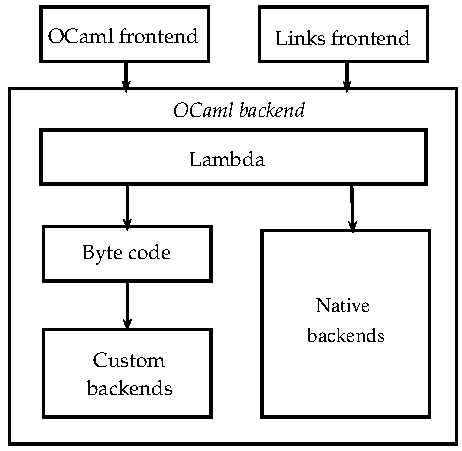
\includegraphics[scale=0.79]{infrastructure-alt.eps}
  \caption{OCaml Backend}\label{fig:infra-diagram}
\end{figure}
We reuse most of the previous Links infrastructure. The Links frontend
is type-checked and translated into a small, typed intermediate
language in \emph{A-normal form} (ANF). The Links interpreter
implements a generalised CEK machine \cite{Hillerstrom2016}, which
interprets ANF code.

Our compilation strategy is to translate the Links ANF language into the OCaml
\emph{Lambda} language, which is a small, untyped lambda calculus. The OCaml
backend exposes a hierarchy of intermediate representations (IRs), where the
top representation is known as Lambda. As shown in the Figure
\ref{fig:infra-diagram}, the Lambda IR offers two different compilation
options: byte code and native code. Therefore by targeting Lambda rather than
a lower level IR, we achieve maximum flexibility as a translation into byte
code, in principle, enables us to take advantage of custom backends such as
\texttt{js\_of\_ocaml} to produce efficient JavaScript.

%
% Alternatively, we could target a lower level IR such as
% \emph{Flambda}, which is an IR intended for high-level
% optimisations. Flambda is reminiscent of the Links IR as it is in
% ANF. However, it is deep into the native compilation pipeline,
% therefore by targetting Lambda rather than Flambda, we achieve maximum
% flexibility as a translation into byte code, in principle, enables us
% to take advantage of custom backends such as \texttt{js\_of\_ocaml} to
% produce JavaScript.

There are several semantic differences between Links and OCaml, e.g. Links
employs structural typing, whilst OCaml predominantly employs nominal typing.
In particular, Links employs row typing for effects, records, and variants,
whereas OCaml only supports row typing for the latter. Exhibiting a faithful
translation from Links to OCaml amounts to a lot of value boxing. Thus, we
target Lambda for greater flexibility and control.  We effectively subvert
OCaml's typechecker by targeting Lambda, however the translation is safe as
Links programs are already typechecked.

% \kc{Mention that the compilation strategy targets OCaml's Lambda intermediate
% code. Mention the reasons behind this choice, which seems unintuitive to a
% casual reader. The reason being that fundamentally, Links' type-system is more
% expressive than OCaml's (row-polymorohism) and hence Links programs cannot be
% faithfully translated to surface OCaml syntax. By targetting Lambda, we subvert
% OCaml's typechecker, but since the Links programs are typechecked already, the
% translation is safe.}

% \begin{figure}
% \begin{tikzpicture}
%   \drawstruct{(4.5,2)}
%   \structcell{\lstinline$do Choose$}  \coordinate (DoChoose) at (currentcell.west);
%   \structcell{$\cdots$}
%   \structcell{\lstinline$do Fail$} \coordinate (DoFail) at (currentcell.east);
%   \structcell{\lstinline$Return-clause$}
%   \structcell{\lstinline[keywordstyle=\footnotesize]$Exception handler$}
%   \structcell{\lstinline$Choose-clause$} \coordinate (HandleChoose1) at (currentcell.west); \coordinate (HandleChoose2) at (currentcell.east);
%   \structcell{$\cdot$} \coordinate (H1) at (currentcell.west);

%   \drawstruct{(0,0)}
%   \structcell{$\cdots$} \coordinate (H2) at (currentcell.east);
%   \structcell{\lstinline$Return-clause$}
%   \structcell{\lstinline[keywordstyle=\footnotesize]$Exception handler$}
%   \structcell{\lstinline$Fail-clause$}
%   \structcell{$\bot$}

% %  \draw[<-] (H2) .. controls ([yshift=0cm] H2) and ([xshift=-10cm,yshift=4cm] H1) .. (H1);
%   \draw (H2) edge[out=-20,in=-175,<-] (H1);
%   \draw (DoChoose) edge[out=175,in=-180,->] (HandleChoose1);
%   \draw (DoFail) edge[xshift=0.5cm,out=0,in=-360,->] (HandleChoose2);
% \end{tikzpicture}
% \caption{Runtime representation of the computation \lstinline$maybeResult(randomResult(drunkToss))$.}\label{fig:rtstack}
% \end{figure}

\section{Runtime representation}
By using the OCaml backend we naturally inherit the OCaml
run-time. OCaml implements effect handlers as heap-managed stack data
structures, and as a consequence composition of handlers gives rise to
$n$-element stacks at run-time. For example, the composition
\lstinline[mathescape]!randomResult(maybeResult($\cdot$))! is
represented as a two-element stack. Thus, an invocation of an abstract
operation amounts to performing a dynamic lookup for a suitable
handler in a stack.

Since the primary use of handlers in OCaml is the express concurrency,
OCaml handlers are affine; continuations can only be resumed at most
once, and multiple invocations of a continuation causes a run-time
error. Multi-shot handlers can be simulated by manually cloning
continuations using \lstinline$Obj.clone_continuation$. The cost of
cloning is linear in the size of the handler stack. However, cloning
is a fragile abstraction; if the handler stack contains at least one
multi-shot handler, then every affine handler in the stack must be
demoted to a multi-shot handler to be safe, because a multi-shot
handler may consume a linear continuation more than
once. Consequently, multi-shot handlers in OCaml break modularity.

In the Links compiler we use the cloning capability under the hood to implement
multi-shot handlers. For example, our encoding of \lstinline$allResults$
amounts to the following in plain OCaml:
% \kc{$Obj.clone$ was too generic and I plan to use $Obj.clone\_continuation$ to
% be less ambiguous.}
\begin{lstlisting}[style=ocaml]
let all_results m = match m () with
 | x -> [x]
 | effect Choose k -> 
   let k' arg = 
     continue (Obj.clone_continuation k) arg 
   in k' true @ k' false
\end{lstlisting}
OCaml provides a unified syntax for pattern-matching on regular, effect, and
exception patterns. The keyword \lstinline[style=ocaml]$effect$ begins an
operation-clause. Essentially, we create a local function \lstinline$k'$, which
wraps the actual continuation \lstinline$k$. An invocation of \lstinline$k'$
passes its argument to a fresh copy of the actual continuation. The
\lstinline$continue$ function is provided by the standard library; given a
continuation and a value, it invokes the continuation with that particular
value. By default we implement every handler as a multi-shot handler.

% \kc{Can we have a small table or something that provides initial results?
% Doesn't need to be extensive. I'd just do Queens, Nim, Chameneos? Otherwise, it
% is unclear what the talk will be about.}.

\begin{table}
  \centering
  \begin{tabular}{| r | r | r | r |}
    \cline{2-4}
    \multicolumn{1}{c|}{~} & \multicolumn{1}{c|}{State} & \multicolumn{1}{c|}{8-Queens} & \multicolumn{1}{c|}{20-Queens}   \\
    \hline
    \multicolumn{1}{|l|}{Interpreter} &  76167&     242  &     411517  \\
    \hline
    \multicolumn{1}{|l|}{Compiler}    &  1619 &        1 &      1059  \\
    \hline
    \multicolumn{1}{|l|}{OCaml (opt)}       &  829  &        1 &       200  \\
    \hline
  \end{tabular}\caption{Micro-benchmarks (execution times are in milliseconds)}\label{tbl:benchmarks}
\end{table}

\section{Optimisations}
% \kc{Rather than talking about this as something you would do in the future, I'd
% write it as current work. In particular, avoid "we plan". I am sure some of
% this work will be done by September. This will form the meat of your actual
% talk I'd think.}
It is rather conservative to implement every handler as multi-shot. We
would like to recover the efficiency of affine handlers, but without
sacrificing the the abstraction. Table \ref{tbl:benchmarks} contains 
the results of a few micro-benchmarks from \citet{Kammar2013}.
% \kc{Even without the optimizations, I expect Links compiled to OCaml to be
% faster than the interpreted version. Compare the performance on Queens? By
% varying the board size:
% https://github.com/kayceesrk/ocaml-eff-example/blob/master/queens.ml}

\paragraph{Linearisation}
Handlers that use their continuations linearly should be promoted to
linear handlers at compile time. We are currently working on applying
the existing linear type system of Links to track the linearity of
handlers.

\paragraph{Handler resolution}
Traversing a large handler stack is likely to be costly. If the
handler stack, or part of it, is known statically, then we can
instantiate abstract operations at compile time.

% \paragraph{Fusion} Handler fusion is a technique to prune the run-time
% stack. Consider the composition
% \lstinline$maybeResult(randomResult(toss))$. It gives
% rise to a stack with two handlers.  We may use row types to guide when
% handler fusion is sound. A necessary criterion for fusion of two
% handlers is that the intersection of their effect signatures is
% empty. We fuse handlers clause by clause, thus for
% \lstinline$maybeResult$ and \lstinline$randomResult$ we obtain:
% \begin{lstlisting}
% sig fused : (Comp({Choose:Bool,Fail:Zero |e}, a)) ->
%              Comp({Choose{_}  ,Fail{_}   |e}, Maybe(a))
% handler fused {
%   case Return(x) -> var y = x; Just(y)
%   case Fail(_)   -> Nothing
%   case Choose(k) -> k(random() > 0.5)
% }
% \end{lstlisting}

% \paragraph{Inlining} Operation inlining enables us to replace abstract
% operations with their implementations, when these are statically
% resolvable. Furthermore, the handler must affine and the operation
% clause must invoke the continuation in tail position. For example, in
% the application \lstinline$randomResult(toss)$ we may replace
% \lstinline$do Choose$ with the computation \lstinline$random() > 0.5$ at compile-time.

\section{Acknowledgements}
The first and second authors were supported by EPSRC grants CDT in
Pervasive Parallelism (EP/L01503X/1) and EP/K034413/1,
respectively.  This work is collaborative work with OCaml Labs.

\bibliographystyle{abbrvnat} \softraggedright
\bibliography{references}

\end{document}
